\documentclass[11pt,a4paper]{article}

% -------------------------------------------------
% PAQUETES BÁSICOS
% -------------------------------------------------
\usepackage[utf8]{inputenc}   % Permite escribir tildes y eñes
\usepackage[T1]{fontenc}
\usepackage[spanish]{babel}    % Traduce nombres automáticos al español
\usepackage{lmodern}
\usepackage{amsmath,amssymb,amsthm}   % Herramientas matemáticas
\usepackage[margin={2.6cm,2.6cm}]{geometry}


\usepackage{fontawesome5}
\usepackage{dirtree}

% -------------------------------------------------
% DATOS DEL DOCUMENTO
% -------------------------------------------------
\title{Guía de LaTeX para principiantes}
\author{Tu nombre}
\date{\today}




% Código fuente
\usepackage{xcolor}
\usepackage{listings}
\usepackage{hyperref}

\definecolor{git}{HTML}{F1502F}
\definecolor{azuluc}{HTML}{1F4E79}

\lstdefinestyle{latexstyle}{
    language=[LaTeX]TeX,
    basicstyle=\ttfamily\small,
    keywordstyle=\color{blue!70!black},
    commentstyle=\color{green!40!black},
    stringstyle=\color{red!70!black},
    %numbers=left,
    numberstyle=\tiny\color{gray},
    numbersep=8pt,
    breaklines=true,
    breakatwhitespace=false,
    frame=single,
    rulecolor=\color{gray!50},
    backgroundcolor=\color{gray!5},
    showstringspaces=false,
    morekeywords={subsection,maketitle,tableofcontents},
    tabsize=4,
    captionpos=b, 
    literate=
    {á}{{\'a}}1
    {é}{{\'e}}1
    {í}{{\'i}}1
    {ó}{{\'o}}1
    {ú}{{\'u}}1
    {Á}{{\'A}}1
    {É}{{\'E}}1
    {Í}{{\'I}}1
    {Ó}{{\'O}}1
    {Ú}{{\'U}}1
    {ñ}{{\~n}}1
    {Ñ}{{\~N}}1
    {ü}{{\"u}}1
    {Ü}{{\"U}}1
    {¡}{{\textexclamdown}}1
	{`}{\textasciigrave}1 
    {´}{\textquotesingle}1,
}

\lstset{style=latexstyle}



% Cajas de contenido
\usepackage[most]{tcolorbox}

\newtcolorbox{paginarecuadrada}[1][]{
    colback=white,
    colframe=black,
    boxrule=0.8pt,
    arc=0mm,
    width=\textwidth,
    left=5mm,
    right=5mm,
    top=5mm,
    bottom=5mm,
    enhanced,
    breakable,
    #1
}




\newtheoremstyle{exercise}{0.8em}{0.8em}{\normalfont}{}{\bfseries\color{azuluc}}{.}{0.5em}{}
\theoremstyle{exercise}
\newtheorem{exercise}{Ejercicio}


\newcommand{\R}{\textcolor{azuluc}{\faIcon{r-project}}}
\newcommand{\Git}{\textcolor{git}{\faIcon{git-alt}}~\!Git}
\newcommand{\GitHub}{\faIcon{github}~\!GitHub}
\newcommand{\Markdown}{Markdown~\faIcon{markdown}}
\newcommand{\checkicon}{\textcolor{verde}{\faIcon{check}}}
\newcommand{\crossicon}{\textcolor{rojo}{\faIcon{times}}}



\title{\LARGE\textbf{Práctica 10: Introducción a \LaTeX}\\[0.5em]
\Large Laboratorio de Matemáticas\\
\small\ \\
\Large Grado en Ingeniería Matemática - Doble Grado en Física e Ingeniería Matemática}
\author{Miguel Beltrá Vidal}
\date{Curso 2026/27}





\begin{document}

\maketitle


\section{Objetivos}

El objetivo de esta práctica es aprender los fundamentos de \LaTeX. Al finalizar, el estudiante deberá ser capaz de crear escribir documentos sencillos con \LaTeX.




% =================================================
% 1. DOCUMENTO EN BLANCO, TÍTULO Y TEXTO
% =================================================

\section{Introducción}

\LaTeX\ es un sistema de preparación y composición de documentos basado en el lenguaje de marcado \TeX, diseñado para crear documentos con una estructura clara, una presentación profesional y una gran calidad tipográfica. 


A diferencia de los procesadores de texto tradicionales, como Microsoft Word, \LaTeX\ no utiliza un sistema de edición WYSIWYG (\emph{What You See Is What You Get}, «lo que ves es lo que obtienes»). En los editores WYSIWYG, el documento se muestra en pantalla prácticamente tal y como aparecerá al imprimirlo o exportarlo, y el usuario puede modificar directamente su apariencia visual. En cambio, \LaTeX\ funciona mediante comandos que indican cómo debe organizarse y presentarse el contenido. El usuario escribe el texto junto con una serie de instrucciones y, posteriormente, el sistema procesa ese código para generar el documento final, habitualmente en formato PDF. Por tanto, se trabaja principalmente sobre el código fuente y no directamente sobre la apariencia visual del documento.

\LaTeX\ es especialmente útil para elaborar documentos que contienen expresiones matemáticas, fórmulas, ecuaciones, tablas, gráficos, referencias bibliográficas y estructuras complejas. Entre sus principales aplicaciones destacan:
\begin{itemize}
	\item \textbf{Documentos académicos:} apuntes, trabajos universitarios, TFG, TFM y tesis doctorales.
	\item \textbf{Publicaciones científicas:} artículos, informes técnicos y comunicaciones para congresos.
	\item \textbf{Documentos matemáticos y científicos:} fórmulas, ecuaciones, demostraciones y notación científica.
	\item \textbf{Libros y manuales:} documentos extensos organizados en capítulos, secciones e índices.
	\item \textbf{Presentaciones:} diapositivas mediante herramientas como Beamer.
\end{itemize}

Una de sus principales ventajas es que permite separar el contenido del formato, facilitando la creación de documentos homogéneos y bien estructurados. Además, automatiza tareas como la numeración de secciones, la generación de índices, la gestión de referencias cruzadas y la elaboración de bibliografías.



\subsection{Ficheros generados}

Al compilar un fichero de \LaTeX\ se generan una serie de ficheros.  Muchos de ellos son ficheros auxiliares que contienen información que servirá para generar el PDF final. Una vez generado dicho PDF, éstos se pueden eliminar. En \Git\ no queremos llevar el seguimiento de estos ficheros intermedios, pues se pueden generar en cualquier momento a partir del código fuente. Revisa el documento sobre \texttt{.gitignore} para ver como excluir dichos ficheros del seguimiento.




% =================================================
% 2. SECCIONES Y TABLA DE CONTENIDOS
% =================================================

%\tableofcontents
%\newpage


\section{Estructura del documento}

\subsection{Clase de documento}\label{sec:documento}

El primer comando que debemos incluir en un documento \LaTeX\ es
\verb|\documentclass|, que permite definir el tipo de documento
que vamos a crear, así como algunas de sus características
generales. La sintaxis general es:

\begin{center}
    \verb|\documentclass[opciones]{clase}|
\end{center}

Las clases de documento más habituales son:

\begin{itemize}
    \item \verb|article|: para artículos, trabajos y documentos
    que no necesitan capítulos.
    \item \verb|proc|: para actas de congresos y publicaciones
    científicas; está basada en la clase \verb|article|.
    \item \verb|minimal|: clase con un formato mínimo, que permite
    construir documentos desde cero.
    \item \verb|report|: para informes y trabajos extensos que
    pueden organizarse en capítulos.
    \item \verb|book|: para libros y documentos organizados en
    capítulos y partes.
\end{itemize}

\noindent Además, podemos especificar algunas opciones para modificar las características del documento:

\begin{itemize}
    \item \verb|10pt|, \verb|11pt|, \verb|12pt|: tamaño de la
    fuente principal del documento.
    \item \verb|a4paper|, \verb|a5paper|, \verb|letterpaper|, etc.:
    tamaño del papel.
    \item \verb|fleqn|: alinea las ecuaciones hacia la izquierda
    en lugar de centrarlas.
    \item \verb|leqno|: coloca los números de las ecuaciones
    en el margen izquierdo.
    \item \verb|titlepage|, \verb|notitlepage|: determina si el
    título aparece en una página independiente.
    \item \verb|onecolumn|, \verb|twocolumn|: establece si el
    documento se presenta en una o dos columnas.
    \item \verb|oneside|, \verb|twoside|: configura el documento
    para impresión a una o a doble cara.
    \item \verb|landscape|: establece la orientación horizontal
    del papel.
    \item \verb|openright|, \verb|openany|: determina si los
    capítulos deben comenzar en una página impar (derecha)
    o en cualquier página.
\end{itemize}

Por ejemplo, podemos crear un documento de tipo artículo,
con papel A4 y un tamaño de fuente de 12 puntos, mediante:

\medskip

\begin{lstlisting}
\documentclass[12pt,a4paper]{article}
\end{lstlisting}


\subsection{Preámbulo}

El preámbulo es la parte del documento comprendida entre \verb|\documentclass| y antes del comando \verb|\begin{document}|. En él se cargan los paquetes necesarios, se definen nuevos comandos y entornos, se configuran diferentes aspectos del documento y se pueden incluir otros archivos de configuración. Algunos de los comandos más habituales son:

\begin{itemize}
    \item \verb|\usepackage[opciones]{paquete}|: carga un paquete que añade funcionalidades a \LaTeX.
    \item \verb|\includeonly{archivos}|: permite seleccionar qué archivos incluidos mediante \verb|\include| se procesarán durante la compilación.
\end{itemize}

\noindent Algunos paquetes habituales son \texttt{amsmath}, \texttt{amssymb}, \texttt{amsfont} o \texttt{amsthm}. También es habitual el paquete \texttt{babel}, que permite configurar el idioma del documento con la opción \texttt{spanish}.

\medskip

Aquí podemos configurar el estilo de las páginas mediante
el comando \verb|\pagestyle|:

\begin{center}
    \verb|\pagestyle{estilo}|
\end{center}

Los estilos más habituales son:

\begin{itemize}
    \item \verb|plain|: muestra el número de página en el pie.
    \item \verb|headings|: muestra información, como el capítulo
    o la sección, junto con el número de página en el encabezado.
    \item \verb|empty|: elimina los encabezados y pies de página,
    incluidos los números de página.
\end{itemize}

También podemos añadir título, autor o fecha del documento con los comandos:


\begin{itemize}
    \item \verb|\title{Titulo del documento}|.
	\item \verb|\author{Nombre del autor}|.
	\item \verb|\date{Fecha del documento}|. Se puede utilizar el comando \verb|\today|.
\end{itemize}

\noindent Para mostrar el título en el documento, deberemos utilizar el comando:
\begin{center}
	\verb|\maketitle|.
\end{center}
donde queramos que aparezca.

\medskip

Un ejemplo típico de preámbulo es el siguiente:

\medskip

\begin{lstlisting}
\documentclass[12pt,a4paper]{article}

\usepackage[spanish]{babel}
\usepackage{amsmath}
\usepackage{amssymb}
\usepackage{amsfonts}
\usepackage{amsthm}

\pagestyle{plain}

\title{Primer ejemplo}
\author{Miguel Beltrá Vidal}
\date{Noviembre 2026}
\end{lstlisting}



\subsection{Documento}

Una vez terminado el preámbulo, añadimos el contenido del documento entre los comandos:

\begin{center}
    \verb|\begin{document}|
    
    \verb|\end{document}|
\end{center}
También podemos dividir el contenido en varios archivos para organizar mejor proyectos extensos. Para ello existen dos comandos principales:

\begin{itemize}
    \item \verb|\include{archivo}|: incorpora el contenido
    de otro archivo \verb|.tex| y comienza una nueva página
    antes de incluirlo.
    \item \verb|\input{archivo}|: incorpora el contenido
    de otro archivo \verb|.tex| directamente, sin forzar
    un salto de página.
\end{itemize}

Por ejemplo, podemos organizar un documento en varios archivos:

\begin{lstlisting}
\documentclass[12pt,a4paper]{report}

\usepackage{amsmath}
\usepackage{amssymb}
\usepackage{amsfonts}
\usepackage{amsthm}

\begin{document}

\include{introduccion}
\include{desarrollo}
\include{conclusiones}

\end{document}
\end{lstlisting}

Los archivos \verb|introduccion.tex|,
\verb|desarrollo.tex| y \verb|conclusiones.tex|
contendrán las distintas partes del documento.


\subsection{Comentarios}

Para añadir comentarios al código de \LaTeX\ se utiliza el carácter \texttt{\%}. El texto que aparece a continuación es ignorado a la hora de generar el documento PDF y sirve para añadir comentarios propios explicativos del código.

\medskip

\begin{lstlisting}
\documentclass[12pt,a4paper]{report}

% Aquí cargamos los paquetes
\usepackage[spanish]{babel} % Configura el idioma del documento
\usepackage{amsmath}
\usepackage{amssymb}
\usepackage{amsfonts}
\usepackage{amsthm}

\begin{document}

\include{introduccion}
\include{desarrollo}
\include{conclusiones}

\end{document}
\end{lstlisting}






\section{Crear secciones}

\LaTeX\ permite organizar el contenido mediante diferentes niveles de división. Los comandos disponibles dependen de la clase de documento utilizada. Los principales comandos de organización son:

\begin{itemize}
    \item \verb|\part{Título}|: crea una parte del documento. Disponible en las clases \verb|book| y \verb|report|.
    \item \verb|\chapter{Título}|: crea un capítulo numerado. Disponible en las clases \verb|book| y \verb|report|, pero no en \verb|article|.
    \item \verb|\section{Título}|: crea una sección numerada.
    \item \verb|\subsection{Título}|: crea una subsección.
    \item \verb|\subsubsection{Título}|: crea una división
    de nivel inferior.
    \item \verb|\paragraph{Título}|: crea un encabezado
    de párrafo.
    \item \verb|\subparagraph{Título}|: crea un encabezado
    de nivel inferior a \verb|\paragraph|.
\end{itemize}

Los comandos de sección también pueden utilizarse con un asterisco para eliminar la numeración automática. Por ejemplo:

\begin{itemize}
    \item \verb|\section*{Título}|
    \item \verb|\subsection*{Título}|
    \item \verb|\subsubsection*{Título}|
\end{itemize}

Estas versiones sin asterisco generan secciones numeradas, mientras que las versiones con asterisco no muestran numeración ni se incorporan automáticamente a la tabla de contenidos. Para generar una tabla de contenidos utilizamos:

\begin{center}
    \verb|\tableofcontents|
\end{center}

Este comando crea automáticamente un índice con los títulos y subtítulos del documento que tengan numeración y estén incluidos en la estructura de secciones. Si queremos añadir manualmente una sección sin numerar a la tabla de contenidos, podemos utilizar:

\medskip

\begin{lstlisting}
\section*{Introducción}
\addcontentsline{toc}{section}{Introducción}
\end{lstlisting}

\medskip

Normalmente \textbf{es necesario compilar el documento dos veces}
para que la tabla de contenidos se genere y actualice
correctamente, incluyendo los títulos y sus números de página.


\subsection{Saltos de páginas}

Podemos empezar una página nueva con el comando:
\begin{center}
	\verb|\newpage|
\end{center}


\section{Enfatizar texto}

\LaTeX permite cambiar el estilo de letra:
\begin{itemize}
	\item \verb|\textbf{...}|: marca el texto en \textbf{negrita}.
	\item \verb|\textit{...}|: marca el texto en \textit{cursiva}.
	\item \verb|\emph{...}|: enfatiza el \emph{texto}.	
\end{itemize}



\newpage
\subsection{Un primer ejemplo}

El código siguiente genera el documento de la página siguiente:

\medskip

\begin{lstlisting}
\documentclass[12pt,a4paper]{article}

\usepackage[spanish]{babel}
\usepackage{amsmath}
\usepackage{amssymb}
\usepackage{amsfonts}
\usepackage{amsthm}

\pagestyle{plain}

\title{Primer ejemplo}
\author{Miguel Beltrá Vidal}
\date{Noviembre 2026}

\begin{document}

\maketitle
\tableofcontents

\section{Primera sección}

Ésta es la sección uno.

\subsection{Primera subsección de la primera sección}

Aquí tenemos una subsección de la sección uno.

\subsection{Segunda subsección de la primera sección}

Aquí tenemos otra subsección de la sección uno.

\section{Segunda sección}

Ésta es la sección dos.

\subsection{Primera subsección de la segunda sección}

Aquí tenemos una subsección de la sección dos.

\end{document}
\end{lstlisting}




\begin{paginarecuadrada}
\begin{center}
	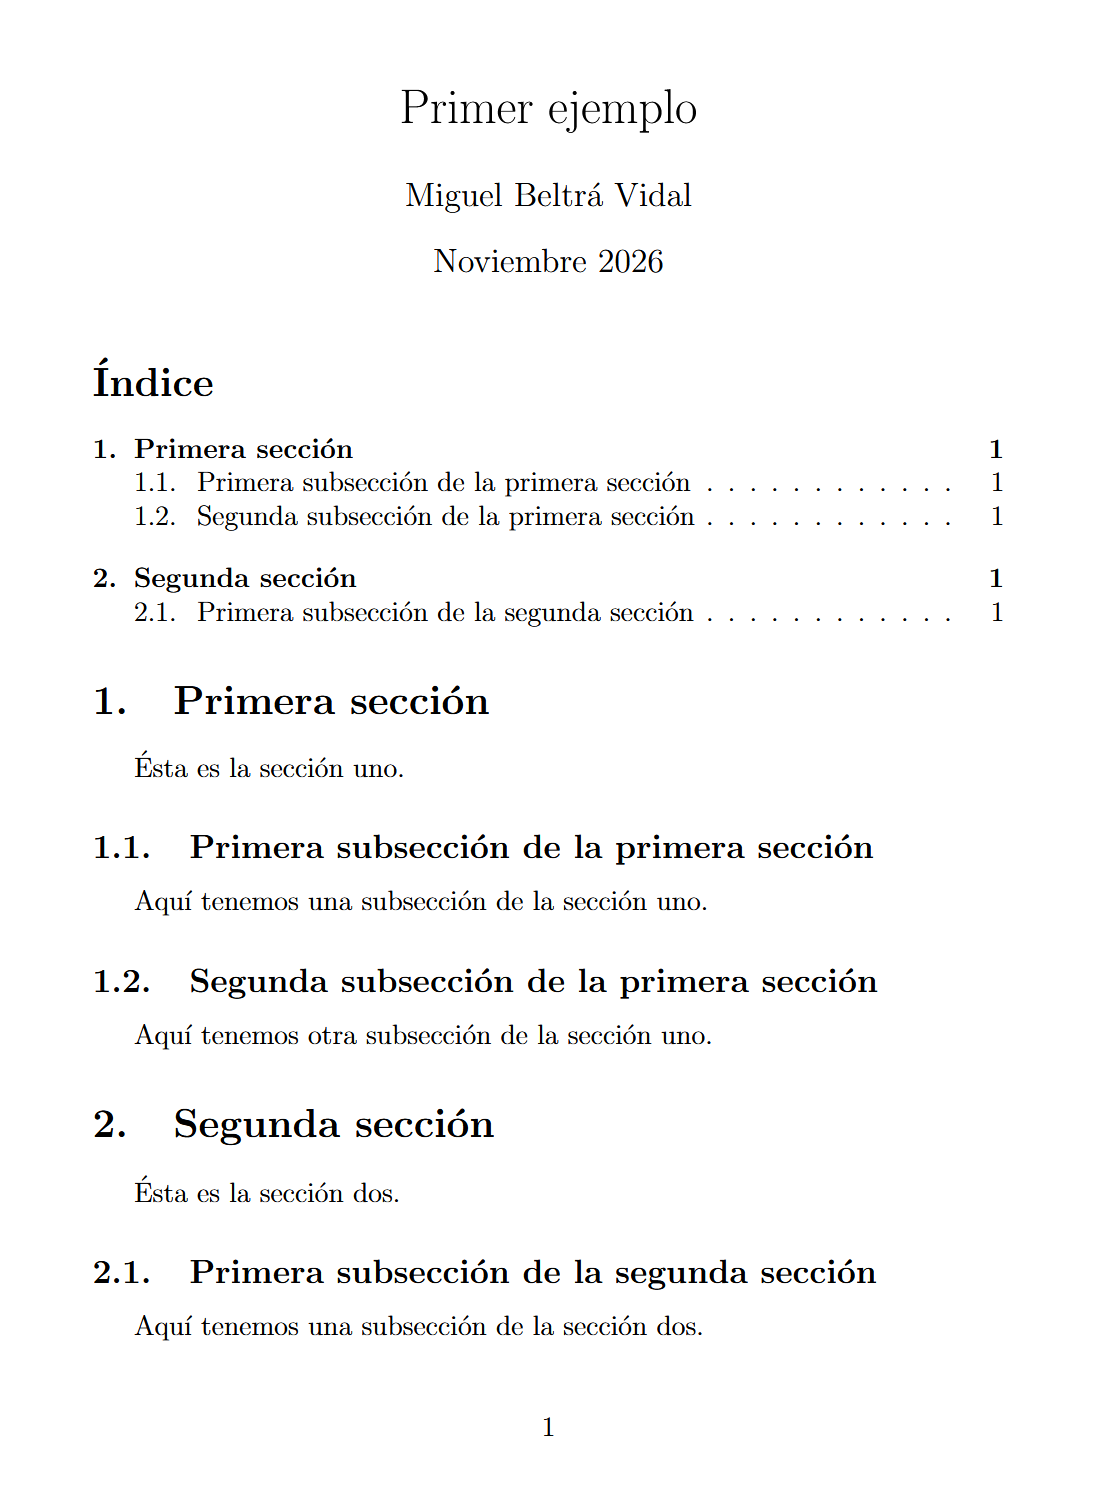
\includegraphics[width=0.95\linewidth]{images/sections.png}
\end{center}
\end{paginarecuadrada}



\newpage
\begin{exercise} Crea un directorio en tu repositorio de prácticas llamado \texttt{LaTeX}. Añade un fichero \texttt{ej1.tex}. Este fichero tendrá el código para generar un documento PDF con formato A4 y tamaño de letra 12, que incluirá lo siguiente:
\begin{enumerate}
	\item Título, autor y fecha de hoy. Además, la página del título deberá aparecer en una página independiente (para ello, mira la sección \ref{sec:documento}).
	
	\item Una tabla de contenidos. En la misma página no habrá nada más (deberás iniciar una nueva página a continuación).
	
	\item Al menos 5 secciones, cada una de ellas con el nombre \textbf{Primera sección}, \textbf{Segunda sección}, etc. Además, añade un texto explicativo similar al del ejemplo: ``Ésta es la sección [número]'', donde en [número] indicarás el número de sección.
	
	 \item Cada sección incluirá 3 subsecciones con un nombre similar a ``\textbf{Primera subsección de la segunda sección}''. Añade un texto descriptivo breve similar al del ejemplo.
	 
	 \item Escoge dos subsecciones entre todas las que tienes. Añade dos subsubsecciones a cada una de ellas y añade un texto descriptivo breve similar a los anteriores.
\end{enumerate}
En tu repositorio de \Git\ deberás llevar un seguimiento tanto del fichero \texttt{ej1.tex} como del documento \texttt{ej1.pdf} generado y subirlo a \GitHub.

\medskip

\noindent \textbf{Atención:} \emph{en la práctica, no es recomendable llevar ningún seguimiento de ningún archivo generable con tu código, como puede ser un fichero PDF, pero en esta asignatura haremos una excepción).}

\end{exercise}














% =================================================
% 3. MODO MATEMÁTICO Y COMANDOS HABITUALES
% =================================================

\section{Modo matemático}

\LaTeX\ tiene un modo especial para escribir expresiones matemáticas.
Hay dos formas habituales de mostrar una fórmula:
\begin{enumerate}
	\item En la misma línea del texto, 
	\begin{itemize}
    		\item Con un signo de dólar: \verb|$ ... $|.
    		\item Con paréntesis escapados: \verb|\( ... \)|.
	\end{itemize}
		
	\item Centrada y separada del texto:
	\begin{itemize}
    		\item Con dos signos de dólar: \verb|$$ ... $$|.
    		\item Con corchetes escapados: \verb|\[ ... \]|.
	\end{itemize}
\end{enumerate}

\noindent \textbf{Es importante líneas en blanco dentro del modo matemático.} Por ejemplo:

\begin{lstlisting}[style=latexstyle]
Esto es una fómula en línea: $a^2+b^2=c^2$. Podemos continuar escribiendo después.

Esto es una fórmula centrada:
\[ e^{i\pi}+1=0. \]
\end{lstlisting}

\noindent El resultado será:

\begin{paginarecuadrada}
Esto es una fómula en línea: $a^2+b^2=c^2$. Podemos continuar escribiendo después.

Esto es una fórmula centrada:
\[
    e^{i\pi}+1=0
\]
\end{paginarecuadrada}

\medskip

\noindent A continuación se listan algunos de los principales símbols matemáticos.

\subsection{Alfabeto griego y algunas letras hebreas}

Las letras griegas se escriben con comandos, exceptuando aquellas que se escriban igual que en el alfabeto latino. Por ejemplo:

\begin{center}
    \begin{tabular}{|cl|cl||cl|cl|} \hline
        Letra & Comando & Letra & Comando & Letra & Comando & Letra & Comando \\ \hline
        A & \verb|A| &
        $\alpha$ & \verb|\alpha| &
	        N & \verb|N| &
	        $\nu$ & \verb|\nu| \\
        B & \verb|B| & 
        $\beta$ & \verb|\beta| &
	        $\Xi$ & \verb|\Xi| &
	        $\xi$ & \verb|\xi| \\
        $\Gamma$ & \verb|\Gamma| &
        $\gamma$ & \verb|\gamma| &
	        O & \verb|O| &
	        o & \verb|o| \\
        $\Delta$ & \verb|\Delta| &
        $\delta$ & \verb|\delta| &
	        $\Pi$ & \verb|\Pi| &
	        $\pi$ & \verb|\pi| \\
        E & \verb|E| &
        $\epsilon$ & \verb|\epsilon| &
	        P & \verb|P| &
	        $\rho$ & \verb|\rho| \\
        Z & \verb|Z| &
        $\zeta$ & \verb|\zeta| &
	        $\Sigma$ & \verb|\Sigma| &
	        $\sigma$ & \verb|\sigma| \\
        H & \verb|H| &
        $\eta$ & \verb|\eta| &
	        T & \verb|T| &
	        $\tau$ & \verb|\tau| \\
        $\Theta$ & \verb|\Theta| &
        $\theta$ & \verb|\theta| &
	        $\Upsilon$ & \verb|\Upsilon| &
	        $\upsilon$ & \verb|\upsilon| \\ 
        I & \verb|I| &
        $\iota$ & \verb|\iota| &
	        $\Phi$ & \verb|\Phi| &
        		$\phi$ & \verb|\phi| \\
        K & \verb|K| &
        $\kappa$ & \verb|\kappa| &
        		X & \verb|X| &
			$\chi$ & \verb|\chi| \\
        $\Lambda$ & \verb|\Lambda| &
        $\lambda$ & \verb|\lambda| &
   	    		$\Psi$ & \verb|\Psi| &
	        $\psi$ & \verb|\psi| \\
        M & \verb|M| &
        $\mu$ & \verb|\mu| &
	        $\omega$ & \verb|\omega| &
	        $\Omega$ & \verb|\Omega| \\ \hline
    \end{tabular}
\end{center}


\noindent Algunas variantes de las letras griegas son las siguientes:

\begin{center}
    \begin{tabular}{|cl|cl|cl|cl|} \hline
        Letra & Comando & Letra & Comando & Letra & Comando & Letra & Comando \\ \hline
        $\varepsilon$ & \verb|\varepsilon| &
        $\vartheta$ & \verb|\vartheta| &
        $\varkappa$ & \verb|\varkappa| &
        $\varpi$ & \verb|\varpi| \\
        $\varrho$ & \verb|\varrho| &
        $\varsigma$ & \verb|\varsigma| &
        $\varphi$ & \verb|\varphi| && \\ \hline
    \end{tabular}
\end{center}


\noindent Letras hebreas:

\begin{center}
    \begin{tabular}{|cl|cl|cl|cl|} \hline
        Letra & Comando & Letra & Comando & Letra & Comando & Letra & Comando \\ \hline
        $\aleph$ & \verb|\aleph| &
        $\beth$ & \verb|\beth| &
        $\gimel$ & \verb|\gimel| &
        $\daleth$ & \verb|\daleth| \\ \hline
    \end{tabular}
\end{center}




\subsection{Operadores y símbolos}

Algunos operadores y símbolos habituales son:

\begin{center}
    \begin{tabular}{|cl|cl|cl|cl|} \hline
        Op. & Comando & Op. & Comando & Op. & Comando & Op. & Comando \\ \hline
        $\times$ & \verb|\times| &
        $\div$ & \verb|\div| &
        $\pm$ & \verb|\pm| &
        $\mp$ & \verb|\mp| \\
        $\oplus$ & \verb|\oplus| &
        $\otimes$ & \verb|\otimes| &
        $\odot$ & \verb|\odot| &
        $\ominus$ & \verb|\ominus| \\
        $\wedge$ & \verb|\wedge| &
        $\vee$ & \verb|\vee| &
        $\neg$ & \verb|\neg| &
        $\bullet$ & \verb|\bullet| \\
        $\cap$ & \verb|\cap| &
        $\cup$ & \verb|\cup| &
        $\setminus$ & \verb|\setminus| &
        $\circ$ & \verb|\circ| \\
        $\int$ & \verb|\int| &
        $\iint$ & \verb|\iint| &
        $\iiint$ & \verb|\iiint| &
        $\oint$ & \verb|\oint| \\ \hline
    \end{tabular}
\end{center}


\noindent Operadores grandes, compatibles con subíndices y superíndices (ver sección \ref{sec:subindices}):

\begin{center}
    \begin{tabular}{|cl|cl|cl|cl|} \hline
        Op. & Comando & Op. & Comando & Op. & Comando & Op. & Comando \\ \hline
        $\bigoplus$ & \verb|\bigoplus| &
        $\bigotimes$ & \verb|\bigotimes| &
        $\bigodot$ & \verb|\bigodot| &
        $\bigcirc$ & \verb|\bigcirc| \\
        $\bigcap$ & \verb|\bigcap| &
        $\bigcup$ & \verb|\bigcup| &
        $\bigwedge$ & \verb|\bigwedge| &
        $\bigvee$ & \verb|\bigvee| \\
        $\sum$ & \verb|\sum| & 
        $\prod$ & \verb|\prod| &
        $\coprod$ & \verb|\coprod| &
        & \\ \hline
    \end{tabular}
\end{center}



\noindent Operadores relacionales:

\begin{center}
    \begin{tabular}{|cl|cl|cl|cl|} \hline
        Op. & Comando & Op. & Comando & Op. & Comando & Op. & Comando \\ \hline
        $\in$ & \verb|\in| & 
        $\notin$ & \verb|\notin| &
        $\ni$ & \verb|\ni| &
        $\neq$ & \verb|\neq| \\
        $\subset$ & \verb|\subset| &
        $\subseteq$ & \verb|\subseteq| &
        $\supset$ & \verb|\supset| &
        $\supseteq$ & \verb|\supseteq| \\
        $\leq$ & \verb|\leq| &
        $\geq$ & \verb|\geq| &
        $\ll$ & \verb|\ll| &
        $\gg$ & \verb|\gg| \\
        $\prec$ & \verb|\prec| &
        $\preceq$ & \verb|\preceq| &
        $\succ$ & \verb|\succ| &
        $\succeq$ & \verb|\succeq| \\
        $\simeq$ & \verb|\simeq| &
        $\approx$ & \verb|\approx| &
        $\cong$ & \verb|\cong| &
        $\equiv$ & \verb|\equiv| \\
        $\propto$ & \verb|\propto| &
        $\mid$ & \verb|\mid| &
        $\nmid$ & \verb|\nmid| & 
        $\parallel$ & \verb|\parallel| \\
        $\perp$ & \verb|\perp| &
        $\top$ & \verb|\top| &
        &&& \\ \hline
    \end{tabular}
\end{center}




\subsection{Flechas}

Algunas flechas frecuentes son:

\begin{center}
    \begin{tabular}{|cl|cl|} \hline
        Flecha & Comando & Flecha & Comando \\ \hline
        $\leftarrow$ & \verb|\leftarrow| &
        $\Leftarrow$ & \verb|\Leftarrow| \\
        $\rightarrow$ & \verb|\rightarrow| &
        $\Rightarrow$ & \verb|\Rightarrow| \\
        $\uparrow$ & \verb|\uparrow| &
        $\Uparrow$ & \verb|\Uparrow| \\
        $\downarrow$ & \verb|\downarrow| &
        $\Downarrow$ & \verb|\Downarrow| \\
        $\leftrightarrow$ & \verb|\leftrightarrow| &
        $\Leftrightarrow$ & \verb|\Leftrightarrow| \\
        $\mapsto$ & \verb|\mapsto| &
        $\nearrow$ & \verb|\nearrow| \\
        $\searrow$ & \verb|\searrow| &
        $\rightleftharpoons$ & \verb|\rightleftharpoons| \\
        $\leftharpoonup$ & \verb|\leftharpoonup| &
        $\rightharpoonup$ & \verb|\rightharpoonup| \\
        $\leftharpoondown$ & \verb|\leftharpoondown| &
        $\rightharpoondown$ & \verb|\rightharpoondown| \\ \hline
    \end{tabular}
\end{center}


\noindent Muchas de estas flechas tiene versión larga:

\begin{center}
    \begin{tabular}{|cl|cl|cl|} \hline
        Flecha & Comando & Flecha & Comando & Flecha & Comando \\ \hline
        $\longleftarrow$ & \verb|\longleftarrow| &
        $\longrightarrow$ & \verb|\longrightarrow| &
        $\longleftrightarrow$ & \verb|\longleftrightarrow| \\
        $\Longleftarrow$ & \verb|\Longleftarrow| &
        $\Longrightarrow$ & \verb|\Longrightarrow| &
        $\Longleftrightarrow$ & \verb|\Longleftrightarrow| \\
        $\longmapsto$ & \verb|\longmapsto| &
        &&&
        \\ \hline
    \end{tabular}
\end{center}


\subsection{Funciones matemáticas}

Algunas funciones matemáticas se escriben con los siguientes comandos:

\begin{center}
    \begin{tabular}{|ll|ll|ll|} \hline
        Func. & Comando & Func. & Comando & Func. & Comando \\ \hline
        $\sin$ & \verb|\sin| &
        $\cos$ & \verb|\cos| &
        $\tan$ & \verb|\tan| \\
        $\arcsin$ & \verb|\arcsin| &
        $\arccos$ & \verb|\arccos| &
        $\arctan$ & \verb|\arctan| \\
        $\csc$ & \verb|\csc| &
        $\sec$ & \verb|\sec| &
        $\cot$ & \verb|\cot| \\
        $\sinh$ & \verb|\sinh| &
        $\cosh$ & \verb|\cosh| &
        $\tanh$ & \verb|\tanh| \\ 
        $\min$ & \verb|\min| &  
        $\max$ & \verb|\max| & 
        $\coth$ & \verb|\coth| \\
        $\inf$ & \verb|\inf| &  
        $\sup$ & \verb|\sup| & 
        $\exp$ & \verb|\exp| \\
        $\log$ & \verb|\log| &
        $\ln$ & \verb|\ln| &
        $\lg$ & \verb|\lg| \\
        $\dim$ & \verb|\dim| &
        $\hom$ & \verb|\hom| &
        $\ker$ & \verb|\ker| \\
        $\det$ & \verb|\det| &
        $\gcd$ & \verb|\gcd| &
        $\lim$ & \verb|\lim| \\ \hline
    \end{tabular}
\end{center}



\subsection{Otros símbolos}


\begin{center}
    \begin{tabular}{|cl|cl|cl|cl|} \hline
        Símb. & Comando & Símb. & Comando & Símb. & Comando & Símb. & Comando \\ \hline
        $\partial$ & \verb|\partial| &
        $\nabla$ & \verb|\nabla| &
        $\emptyset$ & \verb|\emptyset| &
        $\varnothing$ & \verb|\varnothing| \\
        $\forall$ & \verb|\forall| &
        $\exists$ & \verb|\exists| &
        $\nexists$ & \verb|\nexists| &
        $\infty$ & \verb|\infty| \\
        $\Re$ & \verb|\Re| &
        $\Im$ & \verb|\Im| &
        $\wp$ & \verb|\wp| &
        $\surd$ & \verb|\surd| \\
        $\star$ & \verb|\star| &
        $\ell$ & \verb|\ell| &
        $\hbar$ & \verb|\hbar| &
        $\dagger$ & \verb|\dagger| \\
        $\square$ & \verb|\square| &
        $\blacksquare$ & \verb|\blacksquare| &
        $\triangle$ & \verb|\triangle|&
        $\blacktriangle$ & \verb|\blacktriangle| \\ \hline
    \end{tabular}
\end{center}


\noindent Puntos suspensivos:

\begin{center}
	\begin{tabular}{|cl|cl|cl|cl|cl|} \hline
    		Símb. & Com. & Símb. & Com. & Símb. & Com. & Símb. & Com. & Símb. & Com. \\ \hline
        $\cdot$ & \verb|\cdot| &
        $\vdots$ & \verb|\vdots| &
        $\ldots$ & \verb|\ldots| &
        $\cdots$ & \verb|\cdots| &
        $\ddots$ & \verb|\ddots| \\ \hline
    \end{tabular}
\end{center}


\subsection{Tipografías}

Con el comando \verb|\mathcal{...}| tenemos la tipografía:

\[ \mathcal{ABCDEFGHIJKLMNOPQRSTUVWXYZ} \]

Con el comando \verb|\mathfrak{...}| tenemos la tipografía:

\[ \mathfrak{ABCDEFGHIJKLMNOPQRSTUVWXYZ} \]
\[ \mathfrak{abcdefghijklmnopqrstuvwxyz} \]
\[ \mathfrak{0123456789} \]

Con el comando \verb|\mathbb{...}| tenemos la tipografía:

\[ \mathbb{ABCDEFGHIJKLMNOPQRSTUVWXYZ} \]

Con el comando \verb|\mathbf{...}| tenemos la tipografía:

\[ \mathbf{ABCDEFGHIJKLMNOPQRSTUVWXYZ} \]
\[ \mathbf{abcdefghijklmnopqrstuvwxyz} \]
\[ \mathbf{0123456789} \]



\subsection{Carácteres de escape}

Los caracteres \verb|&|, \verb|%|, \verb|$|, \verb|#|, \verb|_|, \verb|{|,\verb|}|, \verb|~|, \verb|^| y \verb|\| tienen un significado especial en \LaTeX, y no se pueden escribir directamente. La siguiente tabla tiene la forma de escribirlos en \LaTeX:
 
 
\begin{center}
	\begin{tabular}{|cl|cl|} \hline
    		Carácter & Comando & Carácter & Comando \\ \hline
        \& & \verb|\&| &
        \% & \verb|\%| \\
        \$ & \verb|\$| &
        \# & \verb|\#| \\
        \{ & \verb|\{| &
        \} & \verb|\}| \\
        \_ & \verb|\_| &
        \textasciicircum & \verb|\textasciicircum| \\
        \textasciitilde  & \verb|\textasciitilde|  &
        \textbackslash   & \verb|\textbackslash| \\ \hline
    \end{tabular}
\end{center}



\subsection{Más símbolos}

Existen multitud de recursos en línea con más símbolos de los que aquí se muestran. Algunos de ellos requerirán de paquetes adicionales que deberás cargar en el preámbulo. Pégale un vistazo a las páginas siguientes:

\begin{enumerate}
	\item \url{https://manualdelatex.com/simbolos}
	\item \url{https://latexmathsymbols.com/}
	\item \url{https://lorca.act.uji.es/curso/latex/documento/symbols-a4.pdf}
	\item \url{https://en.wikipedia.org/wiki/Help:Displaying_a_formula/LaTeX_symbols}
\end{enumerate}





\newpage
\begin{exercise} Crea un fichero llamado \texttt{ej2.tex}. El contenido del fichero debe generar el siguiente documento de \LaTeX. En tu repositorio de \Git\ deberás llevar un seguimiento tanto del fichero \texttt{ej2.tex} como del documento \texttt{ej2.pdf} generado y subirlo a \GitHub.

\vfill
\begin{paginarecuadrada}
\begin{center}
	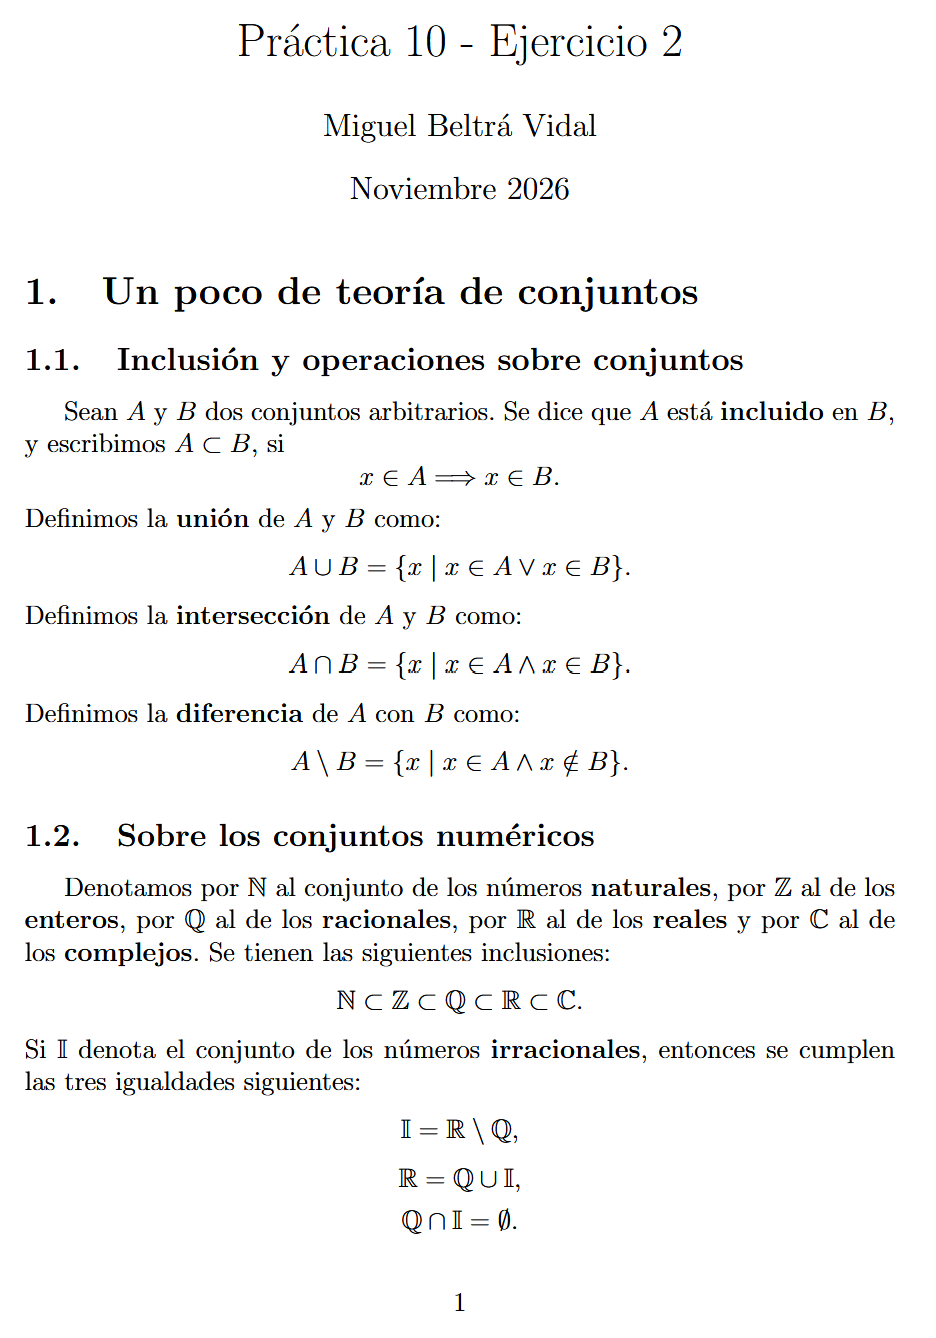
\includegraphics[width=0.9\linewidth]{images/exercise_2.png}
\end{center}
\end{paginarecuadrada}
\vfill
\end{exercise}






% =================================================
% 4. SUBÍNDICES, SUPERÍNDICES Y EXPRESIONES
% =================================================
\newpage
\section{Subíndices, superíndices y otras expresiones frecuentes}\label{sec:subindices}

\subsection{Subíndices y superíndices}

El guion bajo \verb|_| introduce un subíndice y el acento circunflejo \verb|^| introduce un superíndice.

\noindent Por ejemplo, el código siguiente (aquí, \verb|\qquad| representa un espacio en blanco):

\smallskip

\begin{lstlisting}[style=latexstyle]
\[
	x_1   \qquad   x^2   \qquad   x_i^2   \qquad   a_{n+1}
\]
\end{lstlisting}

\smallskip

\noindent El resultado será:

\smallskip

\begin{paginarecuadrada}
\[
x_1 \qquad x^2 \qquad x_i^2 \qquad a_{n+1}
\]
\end{paginarecuadrada}

\smallskip

\noindent Si el subíndice o superíndice contiene más de un carácter,
debes agruparlo entre llaves:

\smallskip

\begin{lstlisting}[style=latexstyle]
\[
	x_{12}   \qquad   x^{n+1}   \qquad a_{ij}^{2n}
\]
\end{lstlisting}

\smallskip

\noindent El resultado será:

\smallskip

\begin{paginarecuadrada}
\[
x_{12} \qquad x^{n+1} \qquad a_{ij}^{2n}
\]
\end{paginarecuadrada}




\subsection{Fracciones}

Para escribir fracciones, se emplea el comando:
\begin{center}
	\verb|\frac{numerador}{denominador}|. 
\end{center}
Si queremos una fracción continua, entonces se emplea el comando:
\begin{center}
	\verb|\cfrac{numerador}{denominador}|. 
\end{center}
Por ejemplo:
\begin{lstlisting}[style=latexstyle]
\[
  \frac{a}{b}  \qquad  \frac{x+1}{x-1}  \qquad  \frac{1}{1+\frac{1}{x}}
  \qquad   \cfrac{1}{1+\cfrac{1}{1+\cfrac{1}{1+\cfrac{1}{x}}}}
\]
\end{lstlisting}

\noindent genera lo siguiente:

\begin{paginarecuadrada}
\[
\frac{a}{b} 
\qquad
\frac{x+1}{x-1} 
\qquad
\frac{1}{1+\frac{1}{x}}
\qquad
\cfrac{1}{1+\cfrac{1}{1+\cfrac{1}{1+\cfrac{1}{x}}}}
\]
\end{paginarecuadrada}



\newpage
\subsection{Raíces}

La raíz cuadrada se escribe con \verb|\sqrt{...}| y la raíz $n$-ésima con \verb|\sqrt[n]{...}|:

\smallskip

\begin{lstlisting}[style=latexstyle]
\[
	\sqrt{x}   \qquad   \sqrt[3]{x+1}
\]
\end{lstlisting}

\smallskip

\noindent genera lo siguiente:

\smallskip

\begin{paginarecuadrada}
\[
\sqrt{x} \qquad \sqrt[3]{x+1}
\]
\end{paginarecuadrada}



\subsection{Sumatorios}
El comando \verb|\sum| crea un sumatorio. Los límites inferior
y superior se indican con subíndice y superíndice. Por ejemplo:

\smallskip

\begin{lstlisting}[style=latexstyle]
\[
	\sum_{i=1}^{n} i   \qquad   \sum_{k=0}^{\infty} \frac{1}{2^k}
\]
\end{lstlisting}

\smallskip

\noindent genera lo siguiente:

\smallskip

\begin{paginarecuadrada}
\[
\sum_{i=1}^{n} i
\qquad
\sum_{k=0}^{\infty} \frac{1}{2^k}
\]
\end{paginarecuadrada}



\subsection{Integrales y límites}
Para una integral se usa \verb|\int|. Los límites se escriben
con \verb|_| y \verb|^|. Por ejemplo:

\smallskip

\begin{lstlisting}[style=latexstyle]
\[
	\int_{a}^{b} f(x) dx   \qquad   \int_{0}^{\infty} e^{-x} dx
\]
\end{lstlisting}

\smallskip

\noindent genera lo siguiente:

\smallskip

\begin{paginarecuadrada}
\[
\int_{a}^{b} f(x)dx
\qquad
\int_{0}^{\infty} e^{-x}dx
\]
\end{paginarecuadrada}

\smallskip


\newpage
El límite de una función se escribe con \verb|\lim| y la flecha de aproximación con \verb|\to|. Por ejemplo:

\smallskip

\begin{lstlisting}[style=latexstyle]
\[
	\lim_{x \to 0} \frac{\sin x}{x}=1
\]
\end{lstlisting}

\smallskip

\noindent genera lo siguiente:

\smallskip

\begin{paginarecuadrada}
\[
\lim_{x\to 0} \frac{\sin x}{x}=1
\]
\end{paginarecuadrada}


\subsection{Uniones, intersecciones y otros símbolos con límites}
Los operadores de conjuntos pueden llevar subíndices y superíndices. Por ejemplo:

\smallskip

\begin{lstlisting}[style=latexstyle]
\[
	\bigcup_{i=1}^{n} A_i   \qquad   \bigcap_{i=1}^{n} A_i
\]
\end{lstlisting}

\smallskip

\noindent genera lo siguiente:

\smallskip

\begin{paginarecuadrada}
\[
\bigcup_{i=1}^{n} A_i
\qquad
\bigcap_{i=1}^{n} A_i
\]
\end{paginarecuadrada}


Otros ejemplos son el producto y el máximo. Por ejemplo:

\smallskip

\begin{lstlisting}[style=latexstyle]
\[
	\prod_{i=1}^{n} a_i   \qquad   \max_{1\leq i\leq n} x_i
\]
\end{lstlisting}

\smallskip

\noindent genera lo siguiente:

\smallskip

\begin{paginarecuadrada}
\[
\prod_{i=1}^{n} a_i   
\qquad
\max_{1\leq i\leq n} x_i
\]
\end{paginarecuadrada}



También puedes escribir una unión sobre todos los conjuntos de una
familia. Por ejemplo:

\smallskip

\begin{lstlisting}[style=latexstyle]
\[
	\bigcup_{i\in I} A_i
\]
\end{lstlisting}

\smallskip

\noindent genera lo siguiente:

\smallskip

\begin{paginarecuadrada}
\[
	\bigcup_{i\in I} A_i
\]
\end{paginarecuadrada}




\subsection{Paréntesis y delimitadores ajustables}
Los comandos \verb|\left| y \verb|\right| ajustan el tamaño
de los delimitadores a la expresión:
\smallskip

\begin{lstlisting}[style=latexstyle]
\[
	\left( \frac{a+b}{c+d} \right)   
	\qquad   
	\left[ \sum_{i=1}^{n} x_i \right]   
	\qquad   
	\left\{ x \in \mathbb{R} : x>0 \right\}.
\]
\end{lstlisting}

\smallskip

\noindent genera lo siguiente:

\smallskip

\begin{paginarecuadrada}
\[
\left( \frac{a+b}{c+d} \right)
\qquad
\left[ \sum_{i=1}^{n} x_i \right]
\qquad
\left\{x\in\mathbb{R}:x>0\right\}
\]
\end{paginarecuadrada}






\newpage
\begin{exercise} Crea un fichero llamado \texttt{ej3.tex}. El contenido del fichero debe generar el siguiente documento de \LaTeX. En tu repositorio de \Git\ deberás llevar un seguimiento tanto del fichero \texttt{ej3.tex} como del documento \texttt{ej3.pdf} generado y subirlo a \GitHub.

\vfill
\begin{paginarecuadrada}
\begin{center}
	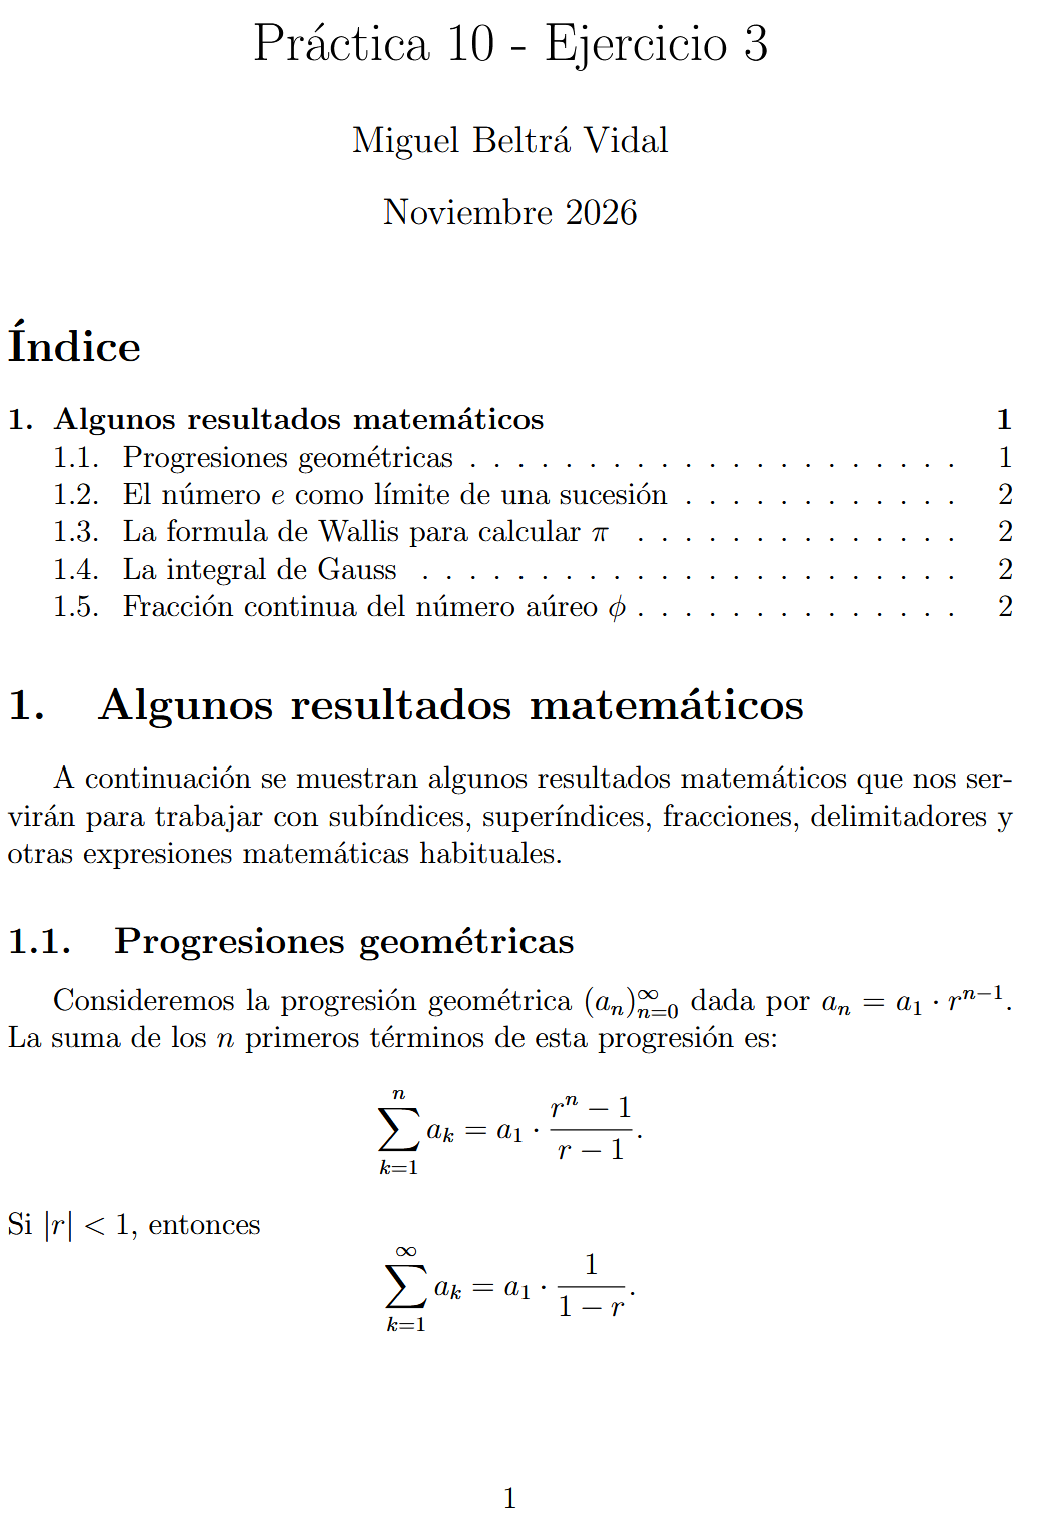
\includegraphics[width=0.9\linewidth]{images/exercise_3_1.png}
\end{center}
\end{paginarecuadrada}
\vfill

\newpage

\vfill
\begin{paginarecuadrada}
\begin{center}
	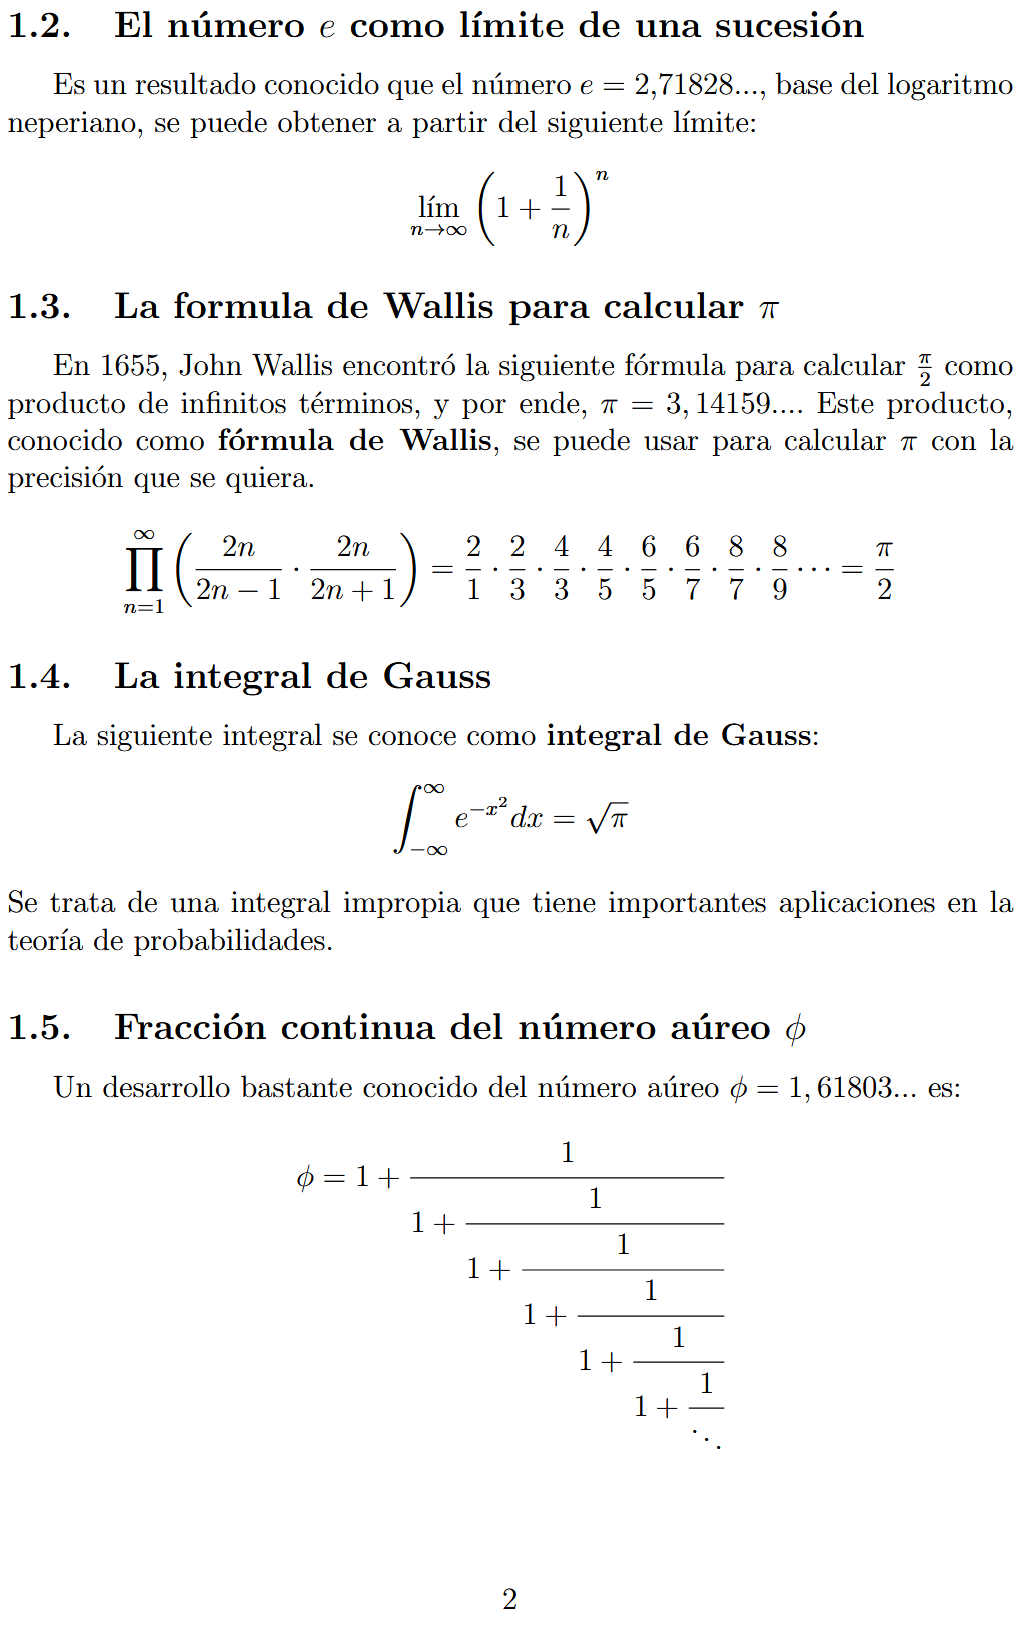
\includegraphics[width=0.9\linewidth]{images/exercise_3_2.png}
\end{center}
\end{paginarecuadrada}
\vfill
\end{exercise}







\section{Documentación del código}

El código debe estar correctamente organizado y comentado. El objetivo no es únicamente conseguir que el PDF se genere correctamente, sino escribir código fácil de leer y modificar.


\begin{exercise} Crea un fichero \texttt{README.md} para documentar esta práctica. El aspecto deberá ser similar al de las prácticas anteriores.
\end{exercise}


\section{Entrega}

Sube los ficheros con los ejercicios a tu \GitHub\ en la fecha acordada con el profesor. Para esta práctica:
\begin{enumerate}
	\item guarda tus ficheros \texttt{.tex} en la carpeta de la práctica correspondiente;
	\item utiliza nombres de fichero claros y consistentes;
	\item comprueba que el documento \texttt{.pdf} se genera correctamente.
\end{enumerate}
Después de esta práctica, la estructura de directorios de tu repositorio se debería parecer a la siguiente:

\begin{center}
\begin{minipage}{0.75\linewidth}
\dirtree{%
    .1 \faIcon[regular]{folder-open}\ practicas/.
	    .2 \faIcon[regular]{folder-open}\ .git/.
        .2 \faIcon[regular]{folder-open}\ assets/.
            .3 \faIcon[regular]{folder-open}\ images/.
        .2 \faIcon[regular]{folder-open}\ Git/.
        .2 \faIcon[regular]{folder-open}\ R/.
        .2 \faIcon[regular]{folder-open}\ LaTeX/.
        		.3 \faIcon[regular]{folder-open}\ practica\_10/.
		        .4 \faIcon[regular]{file-alt}\ ej1.tex.
		        .4 \faIcon[regular]{file-pdf}\ ej1.pdf.
		        .4 \faIcon[regular]{file-alt}\ ej2.tex.
		        .4 \faIcon[regular]{file-pdf}\ ej2.pdf.
		        .4 \faIcon[regular]{file-alt}\ ej3.tex.
		        .4 \faIcon[regular]{file-pdf}\ ej3.pdf.
		        .4 \faIcon[regular]{file-alt}\ README.md.
        .2 \faIcon[regular]{file-alt}\ .gitignore.
        .2 \faIcon[regular]{file-alt}\ README.md.
}
\end{minipage}
\end{center}




\end{document}
